\documentclass[]{scrartcl}
\usepackage{Preamble}

\setcounter{section}{3}
\newcommand{\exercise}{Exercise \thesection}
\newcommand{\duedate}{2020-11-30, 23:59}

\begin{document}
\section*{\exercise}

To compile: unzip our uploaded code, and run \verb|make| inside \verb|code/|.
The slurm scripts are stored inside \verb|code/slurm/|.

\subsection{Measure Latency}
The MPI ping-pong implementation in \verb|code/src/latency.cpp| is measuring the roundtrip latency for each ping pong exchange 100000 times.
This results in the latencies observed in \autoref{fig:latency}.
Visualized in blue are the times for two ranks running on the same node, while the communication between two ranks on two different nodes is visualized in red.

\begin{figure}[ht]
    \centering
    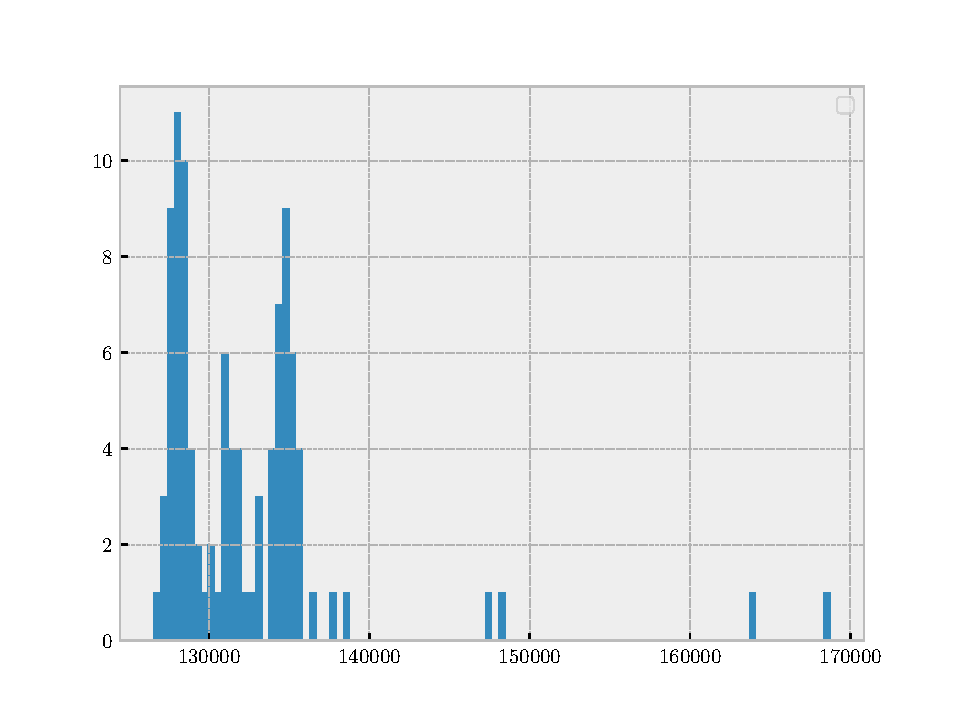
\includegraphics[width=\linewidth]{img/latency}
    \caption{Roundtrip Latency over 100000 ping-pong exchanges}%
    \label{fig:latency}
\end{figure}

Both times the Latency roughly increases linearly with message size and for the communication between nodes a distinct offset and worse latency scaling can be observed

\subsection{Measure Bandwidth}
The MPI flood-test implentation in \verb|code/src/bandwidth.cpp| is measuring the bandwidth over an averarge of 1000 mags, repeating this measurement 100 times.
This results in the bandwidths observed in \autoref{fig:bandwidth}.

\begin{figure}[ht]
    \centering
    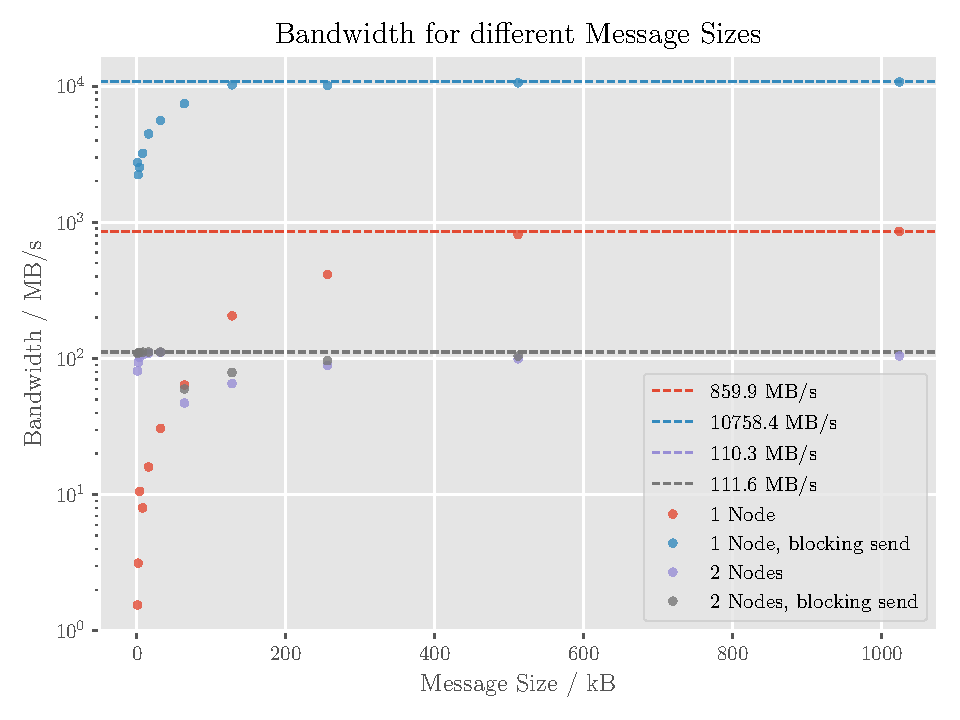
\includegraphics[width=\linewidth]{img/bandwidth}
    \caption{Bandwidth over 100000 flood-messages}%
    \label{fig:bandwidth}
\end{figure}
\subsection{Matrix multiply --- sequential}
\end{document}
